%% bare_conf.tex
%% V1.3
%% 2007/01/11
%% by Michael Shell
%% See:
%% http://www.michaelshell.org/
%% for current contact information.
%%
%% This is a skeleton file demonstrating the use of IEEEtran.cls
%% (requires IEEEtran.cls version 1.7 or later) with an IEEE conference paper.
%%
%% Support sites:
%% http://www.michaelshell.org/tex/ieeetran/
%% http://www.ctan.org/tex-archive/macros/latex/contrib/IEEEtran/
%% and
%% http://www.ieee.org/

%%*************************************************************************
%% Legal Notice:
%% This code is offered as-is without any warranty either expressed or
%% implied; without even the implied warranty of MERCHANTABILITY or
%% FITNESS FOR A PARTICULAR PURPOSE! 
%% User assumes all risk.
%% In no event shall IEEE or any contributor to this code be liable for
%% any damages or losses, including, but not limited to, incidental,
%% consequential, or any other damages, resulting from the use or misuse
%% of any information contained here.
%%
%% All comments are the opinions of their respective authors and are not
%% necessarily endorsed by the IEEE.
%%
%% This work is distributed under the LaTeX Project Public License (LPPL)
%% ( http://www.latex-project.org/ ) version 1.3, and may be freely used,
%% distributed and modified. A copy of the LPPL, version 1.3, is included
%% in the base LaTeX documentation of all distributions of LaTeX released
%% 2003/12/01 or later.
%% Retain all contribution notices and credits.
%% ** Modified files should be clearly indicated as such, including  **
%% ** renaming them and changing author support contact information. **
%%
%% File list of work: IEEEtran.cls, IEEEtran_HOWTO.pdf, bare_adv.tex,
%%                    bare_conf.tex, bare_jrnl.tex, bare_jrnl_compsoc.tex
%%*************************************************************************

% *** Authors should verify (and, if needed, correct) their LaTeX system  ***
% *** with the testflow diagnostic prior to trusting their LaTeX platform ***
% *** with production work. IEEE's font choices can trigger bugs that do  ***
% *** not appear when using other class files.                            ***
% The testflow support page is at:
% http://www.michaelshell.org/tex/testflow/



% Note that the a4paper option is mainly intended so that authors in
% countries using A4 can easily print to A4 and see how their papers will
% look in print - the typesetting of the document will not typically be
% affected with changes in paper size (but the bottom and side margins will).
% Use the testflow package mentioned above to verify correct handling of
% both paper sizes by the user's LaTeX system.
%
% Also note that the "draftcls" or "draftclsnofoot", not "draft", option
% should be used if it is desired that the figures are to be displayed in
% draft mode.
%
\documentclass[conference,10pt,us]{IEEEtran}
% Add the compsoc option for Computer Society conferences.
%
% If IEEEtran.cls has not been installed into the LaTeX system files,
% manually specify the path to it like:
% \documentclass[conference]{../sty/IEEEtran}




% Some very useful LaTeX packages include:
% (uncomment the ones you want to load)


% *** MISC UTILITY PACKAGES ***
%
%\usepackage{ifpdf}
% Heiko Oberdiek's ifpdf.sty is very useful if you need conditional
% compilation based on whether the output is pdf or dvi.
% usage:
% \ifpdf
%   % pdf code
% \else
%   % dvi code
% \fi
% The latest version of ifpdf.sty can be obtained from:
% http://www.ctan.org/tex-archive/macros/latex/contrib/oberdiek/
% Also, note that IEEEtran.cls V1.7 and later provides a builtin
% \ifCLASSINFOpdf conditional that works the same way.
% When switching from latex to pdflatex and vice-versa, the compiler may
% have to be run twice to clear warning/error messages.






% *** CITATION PACKAGES ***
%
%\usepackage{cite}
% cite.sty was written by Donald Arseneau
% V1.6 and later of IEEEtran pre-defines the format of the cite.sty package
% \cite{} output to follow that of IEEE. Loading the cite package will
% result in citation numbers being automatically sorted and properly
% "compressed/ranged". e.g., [1], [9], [2], [7], [5], [6] without using
% cite.sty will become [1], [2], [5]--[7], [9] using cite.sty. cite.sty's
% \cite will automatically add leading space, if needed. Use cite.sty's
% noadjust option (cite.sty V3.8 and later) if you want to turn this off.
% cite.sty is already installed on most LaTeX systems. Be sure and use
% version 4.0 (2003-05-27) and later if using hyperref.sty. cite.sty does
% not currently provide for hyperlinked citations.
% The latest version can be obtained at:
% http://www.ctan.org/tex-archive/macros/latex/contrib/cite/
% The documentation is contained in the cite.sty file itself.






% *** GRAPHICS RELATED PACKAGES ***
%
\ifCLASSINFOpdf
  \usepackage[pdftex]{graphicx}
  % declare the path(s) where your graphic files are
  % \graphicspath{{../pdf/}{../jpeg/}}
  % and their extensions so you won't have to specify these with
  % every instance of \includegraphics
  % \DeclareGraphicsExtensions{.pdf,.jpeg,.png}
\else
  % or other class option (dvipsone, dvipdf, if not using dvips). graphicx
  % will default to the driver specified in the system graphics.cfg if no
  % driver is specified.
  % \usepackage[dvips]{graphicx}
  % declare the path(s) where your graphic files are
  % \graphicspath{{../eps/}}
  % and their extensions so you won't have to specify these with
  % every instance of \includegraphics
  % \DeclareGraphicsExtensions{.eps}
\fi
% graphicx was written by David Carlisle and Sebastian Rahtz. It is
% required if you want graphics, photos, etc. graphicx.sty is already
% installed on most LaTeX systems. The latest version and documentation can
% be obtained at: 
% http://www.ctan.org/tex-archive/macros/latex/required/graphics/
% Another good source of documentation is "Using Imported Graphics in
% LaTeX2e" by Keith Reckdahl which can be found as epslatex.ps or
% epslatex.pdf at: http://www.ctan.org/tex-archive/info/
%
% latex, and pdflatex in dvi mode, support graphics in encapsulated
% postscript (.eps) format. pdflatex in pdf mode supports graphics
% in .pdf, .jpeg, .png and .mps (metapost) formats. Users should ensure
% that all non-photo figures use a vector format (.eps, .pdf, .mps) and
% not a bitmapped formats (.jpeg, .png). IEEE frowns on bitmapped formats
% which can result in "jaggedy"/blurry rendering of lines and letters as
% well as large increases in file sizes.
%
% You can find documentation about the pdfTeX application at:
% http://www.tug.org/applications/pdftex





% *** MATH PACKAGES ***
%
%\usepackage[cmex10]{amsmath}
% A popular package from the American Mathematical Society that provides
% many useful and powerful commands for dealing with mathematics. If using
% it, be sure to load this package with the cmex10 option to ensure that
% only type 1 fonts will utilized at all point sizes. Without this option,
% it is possible that some math symbols, particularly those within
% footnotes, will be rendered in bitmap form which will result in a
% document that can not be IEEE Xplore compliant!
%
% Also, note that the amsmath package sets \interdisplaylinepenalty to 10000
% thus preventing page breaks from occurring within multiline equations. Use:
%\interdisplaylinepenalty=2500
% after loading amsmath to restore such page breaks as IEEEtran.cls normally
% does. amsmath.sty is already installed on most LaTeX systems. The latest
% version and documentation can be obtained at:
% http://www.ctan.org/tex-archive/macros/latex/required/amslatex/math/





% *** SPECIALIZED LIST PACKAGES ***
%
%\usepackage{algorithmic}
% algorithmic.sty was written by Peter Williams and Rogerio Brito.
% This package provides an algorithmic environment fo describing algorithms.
% You can use the algorithmic environment in-text or within a figure
% environment to provide for a floating algorithm. Do NOT use the algorithm
% floating environment provided by algorithm.sty (by the same authors) or
% algorithm2e.sty (by Christophe Fiorio) as IEEE does not use dedicated
% algorithm float types and packages that provide these will not provide
% correct IEEE style captions. The latest version and documentation of
% algorithmic.sty can be obtained at:
% http://www.ctan.org/tex-archive/macros/latex/contrib/algorithms/
% There is also a support site at:
% http://algorithms.berlios.de/index.html
% Also of interest may be the (relatively newer and more customizable)
% algorithmicx.sty package by Szasz Janos:
% http://www.ctan.org/tex-archive/macros/latex/contrib/algorithmicx/




% *** ALIGNMENT PACKAGES ***
%
%\usepackage{array}
% Frank Mittelbach's and David Carlisle's array.sty patches and improves
% the standard LaTeX2e array and tabular environments to provide better
% appearance and additional user controls. As the default LaTeX2e table
% generation code is lacking to the point of almost being broken with
% respect to the quality of the end results, all users are strongly
% advised to use an enhanced (at the very least that provided by array.sty)
% set of table tools. array.sty is already installed on most systems. The
% latest version and documentation can be obtained at:
% http://www.ctan.org/tex-archive/macros/latex/required/tools/


%\usepackage{mdwmath}
%\usepackage{mdwtab}
% Also highly recommended is Mark Wooding's extremely powerful MDW tools,
% especially mdwmath.sty and mdwtab.sty which are used to format equations
% and tables, respectively. The MDWtools set is already installed on most
% LaTeX systems. The lastest version and documentation is available at:
% http://www.ctan.org/tex-archive/macros/latex/contrib/mdwtools/


% IEEEtran contains the IEEEeqnarray family of commands that can be used to
% generate multiline equations as well as matrices, tables, etc., of high
% quality.


%\usepackage{eqparbox}
% Also of notable interest is Scott Pakin's eqparbox package for creating
% (automatically sized) equal width boxes - aka "natural width parboxes".
% Available at:
% http://www.ctan.org/tex-archive/macros/latex/contrib/eqparbox/





% *** SUBFIGURE PACKAGES ***
%\usepackage[tight,footnotesize]{subfigure}
% subfigure.sty was written by Steven Douglas Cochran. This package makes it
% easy to put subfigures in your figures. e.g., "Figure 1a and 1b". For IEEE
% work, it is a good idea to load it with the tight package option to reduce
% the amount of white space around the subfigures. subfigure.sty is already
% installed on most LaTeX systems. The latest version and documentation can
% be obtained at:
% http://www.ctan.org/tex-archive/obsolete/macros/latex/contrib/subfigure/
% subfigure.sty has been superceeded by subfig.sty.



%\usepackage[caption=false]{caption}
%\usepackage[font=footnotesize]{subfig}
% subfig.sty, also written by Steven Douglas Cochran, is the modern
% replacement for subfigure.sty. However, subfig.sty requires and
% automatically loads Axel Sommerfeldt's caption.sty which will override
% IEEEtran.cls handling of captions and this will result in nonIEEE style
% figure/table captions. To prevent this problem, be sure and preload
% caption.sty with its "caption=false" package option. This is will preserve
% IEEEtran.cls handing of captions. Version 1.3 (2005/06/28) and later 
% (recommended due to many improvements over 1.2) of subfig.sty supports
% the caption=false option directly:
%\usepackage[caption=false,font=footnotesize]{subfig}
%
% The latest version and documentation can be obtained at:
% http://www.ctan.org/tex-archive/macros/latex/contrib/subfig/
% The latest version and documentation of caption.sty can be obtained at:
% http://www.ctan.org/tex-archive/macros/latex/contrib/caption/




% *** FLOAT PACKAGES ***
%
%\usepackage{fixltx2e}
% fixltx2e, the successor to the earlier fix2col.sty, was written by
% Frank Mittelbach and David Carlisle. This package corrects a few problems
% in the LaTeX2e kernel, the most notable of which is that in current
% LaTeX2e releases, the ordering of single and double column floats is not
% guaranteed to be preserved. Thus, an unpatched LaTeX2e can allow a
% single column figure to be placed prior to an earlier double column
% figure. The latest version and documentation can be found at:
% http://www.ctan.org/tex-archive/macros/latex/base/



%\usepackage{stfloats}
% stfloats.sty was written by Sigitas Tolusis. This package gives LaTeX2e
% the ability to do double column floats at the bottom of the page as well
% as the top. (e.g., "\begin{figure*}[!b]" is not normally possible in
% LaTeX2e). It also provides a command:
%\fnbelowfloat
% to enable the placement of footnotes below bottom floats (the standard
% LaTeX2e kernel puts them above bottom floats). This is an invasive package
% which rewrites many portions of the LaTeX2e float routines. It may not work
% with other packages that modify the LaTeX2e float routines. The latest
% version and documentation can be obtained at:
% http://www.ctan.org/tex-archive/macros/latex/contrib/sttools/
% Documentation is contained in the stfloats.sty comments as well as in the
% presfull.pdf file. Do not use the stfloats baselinefloat ability as IEEE
% does not allow \baselineskip to stretch. Authors submitting work to the
% IEEE should note that IEEE rarely uses double column equations and
% that authors should try to avoid such use. Do not be tempted to use the
% cuted.sty or midfloat.sty packages (also by Sigitas Tolusis) as IEEE does
% not format its papers in such ways.





% *** PDF, URL AND HYPERLINK PACKAGES ***
%
%\usepackage{url}
% url.sty was written by Donald Arseneau. It provides better support for
% handling and breaking URLs. url.sty is already installed on most LaTeX
% systems. The latest version can be obtained at:
% http://www.ctan.org/tex-archive/macros/latex/contrib/misc/
% Read the url.sty source comments for usage information. Basically,
% \url{my_url_here}.





% *** Do not adjust lengths that control margins, column widths, etc. ***
% *** Do not use packages that alter fonts (such as pslatex).         ***
% There should be no need to do such things with IEEEtran.cls V1.6 and later.
% (Unless specifically asked to do so by the journal or conference you plan
% to submit to, of course. )


% correct bad hyphenation here
\hyphenation{op-tical net-works semi-conduc-tor}

\usepackage{pgfplots}
\pgfplotsset{compat=1.8}
\usepgfplotslibrary{groupplots}
\usepackage{tikz}
\usetikzlibrary{patterns}
\usepackage{booktabs}
\usepackage{multirow}
\usepackage{url}
\usepackage{amsmath}
\usepackage{amsthm}
\usepackage{amsfonts}
\usepackage{subfig}
\usepackage{graphicx}
\usepackage{epstopdf}
\usepackage[boxed,linesnumberedhidden]{algorithm2e}
\pagestyle{empty}
\newtheorem{theorem}{Theorem}[section]
\newtheorem{lemma}[theorem]{Lemma}
\newtheorem{proposition}[theorem]{Proposition}
\newtheorem{corollary}[theorem]{Corollary}
\usepackage{mdwlist}
% \usepackage{bibspacing}
\usepackage{color}
\makeatletter
\newbox\sf@box
\newenvironment{SubFloat}[2][]%
{\def\sf@one{#1}%
\def\sf@two{#2}%
\setbox\sf@box\hbox
\bgroup}%
{ \egroup
\ifx\@empty\sf@two\@empty\relax
\def\sf@two{\@empty}
\fi
\ifx\@empty\sf@one\@empty\relax
\subfloat[\sf@two]{\box\sf@box}%
\else
\subfloat[\sf@one][\sf@two]{\box\sf@box}%
\fi}
\makeatother

\begin{document}
%
% paper title
% can use linebreaks \\ within to get better formatting as desired
% \title{Bare Demo of IEEEtran.cls for Conferences}
\title{Times square -- an intersection of logical and physical
  times} % Modified by K. Kobayashi 18/06/02


% author names and affiliations
% use a multiple column layout for up to three different
% affiliations
\author{}

% conference papers do not typically use \thanks and this command
% is locked out in conference mode. If really needed, such as for
% the acknowledgment of grants, issue a \IEEEoverridecommandlockouts
% after \documentclass

% for over three affiliations, or if they all won't fit within the width
% of the page, use this alternative format:
% 
%\author{\IEEEauthorblockN{Michael Shell\IEEEauthorrefmark{1},
%Homer Simpson\IEEEauthorrefmark{2},
%James Kirk\IEEEauthorrefmark{3}, 
%Montgomery Scott\IEEEauthorrefmark{3} and
%Eldon Tyrell\IEEEauthorrefmark{4}}
%\IEEEauthorblockA{\IEEEauthorrefmark{1}School of Electrical and Computer Engineering\\
%Georgia Institute of Technology,
%Atlanta, Georgia 30332--0250\\ Email: see http://www.michaelshell.org/contact.html}
%\IEEEauthorblockA{\IEEEauthorrefmark{2}Twentieth Century Fox, Springfield, USA\\
%Email: homer@thesimpsons.com}
%\IEEEauthorblockA{\IEEEauthorrefmark{3}Starfleet Academy, San Francisco, California 96678-2391\\
%Telephone: (800) 555--1212, Fax: (888) 555--1212}
%\IEEEauthorblockA{\IEEEauthorrefmark{4}Tyrell Inc., 123 Replicant Street, Los Angeles, California 90210--4321}}




% use for special paper notices
%\IEEEspecialpapernotice{(Invited Paper)}




% make the title area
\maketitle


\begin{abstract}
%\boldmath
  In this paper we introduce deterministic and non-deterministic
  real-time delay into reactive Globally Asynchronous Locally
  Synchronous (GALS) programming languages and synchronous languages as
  their constituent part. The language constructs that allow use of
  real-time delay are illustrated on the SystemJ GALS language. They
  allow system designers to explicitly use, at the specification level,
  not only logical time but also the real-time in order to control
  system operation. The introduced concepts utilize execution platforms
  that allow finding best and worst periods of the logical clock of a
  GALS or synchronous program.
\end{abstract}
% IEEEtran.cls defaults to using nonbold math in the Abstract.
% This preserves the distinction between vectors and scalars. However,
% if the conference you are submitting to favors bold math in the abstract,
% then you can use LaTeX's standard command \boldmath at the very start
% of the abstract to achieve this. Many IEEE journals/conferences frown on
% math in the abstract anyway.

% no keywords




% For peer review papers, you can put extra information on the cover
% page as needed:
% \ifCLASSOPTIONpeerreview
% \begin{center} \bfseries EDICS Category: 3-BBND \end{center}
% \fi
%
% For peerreview papers, this IEEEtran command inserts a page break and
% creates the second title. It will be ignored for other modes.
\IEEEpeerreviewmaketitle

\section{Introduction and motivation}
\label{sec:intr-motiv}

Reactive languages~\cite{gber931,amal10} are a class of programming
languages used for designing and implementing reactive systems, which
continuously respond to input from their environment. These languages
have been successfully used in programming a plethora of systems such as
fly-by-wire in Airbus~\cite{eairbus}, security surveillance
systems~\cite{amal121}, etc. Usually these systems also need to meet
real-time constraints enforced by the environment. Yet, these languages
do not support describing real-time statements as first class language
constructs.  For example, one cannot describe a simple real-time delay
(postponement) of an operation for 0.2 ms. These languages are based on
formal semantics, essential for the formal reasoning about and
verification of correctness of functional properties of the developed
programs, but leave nonfunctional properties such as timing behavior as
an implementation detail~\cite{boldt07}. Arguably, rightly so, because
physical time cannot be incorporated without information about the
underlying execution platform.  But, one can still reason in terms of
logical time. These languages support discrete logical clock rather than
a discrete physical (real-time) clock. The real-time period of the
discrete logical clock (also referred to as a logical tick) is not fixed
and it is determined by the responsiveness of the program to the input
signals. Unlike a discrete physical clock, which has fixed real-time
period, the period of the logical clock is elastic. Although the timing
model with logical clock has worked well for reactive synchronous/GALS
languages in designing discrete systems, there is a need to introduce
real-time since, often, implementation models are in the continuous or
discrete real-time domain~\cite{DBLP:journals/pieee/SifakisTY03}.
Moreover, adding timing capabilities as first class language constructs
create additional opportunity for formally verifying functional and
non-functional requirements before system deployment.

\subsection{Motivating Example}
\label{sec:motivating-example}

% system{
%  interface{
%   input signal TOUCH;
%   output signal GREEN_LIGHT;
%   output char channel S;
%   input char channel R;
%  }
\begin{figure}[t!]
% \begin{center}
\begin{minipage}{5cm}
  \begin{scriptsize}
    
\begin{verbatim}
{ // Clock-domain 1
while(true) {
  trap(TRAP){
   // Abort if user touches the screen
   abort(TOUCH){
    {sustain GREEN_LIGHT;}
    || // synchronous parallel operator
    {
     //exit after any where from 50.3 to 200.3 ms.
     delay (50.3 .. 200.3 ms);
     exit(TRAP); 
    }
   } do {send S(1);} // Send 1 if touched 
  } do {send S(0);} // Else Send 0
  pause; // only construct to consume time
 }
}
>< // asynchronous operator
{ // Clock-domain 2
  while(true){ receive S; // do something with S}
}
\end{verbatim}
  \end{scriptsize}
\end{minipage}
\caption{An example human responsiveness system (HRTCS)}
% }
% \end{center}
\label{fig:1}
\end{figure}

Consider a simple machine used to test human response time and collect
this data for future research purposes. The machine switches on a green
light on a touch screen for anywhere between 50.3 ms to 200.3 ms, if the
user can touch this green light then she is successful and an integer
\texttt{1} is sent to a database, if unsuccessful a \texttt{0} is sent
instead, Different statistics and analyses on human responsiveness can
be based on collected data.

The SystemJ pseudo-code~\cite{amal10} for such a system is shown in
Figure~\ref{fig:1}. We use the SystemJ language in this paper, first of
all, because being a \textit{Globally Asynchronous Locally Synchronous}
(GALS) language it helps us easily describe a larger class of systems
(like HRTCS in Figure~\ref{fig:1}) compared to purely synchronous
languages like Esterel. Moreover, being a super-set of Esterel, SystemJ
allows us to explore the marriage of real-time and logical time, which
is equally applicable to the synchronous sub-set.

The SystemJ program is divided into two clock-domains, the first
clock-domain continuously displays a green light (\texttt{GREEN\_LIGHT}
signal) on the touch screen sensor and waits for the user to respond. If
the user is able to touch the screen within the specified time of 50.3
ms to 200.3 ms a positive response is sent to the second
clock-domain. All the SystemJ programming constructs used to implement
this system are described in~\cite{amal10} and Table~\ref{tab:1} in
Section~\ref{sec:background}. The delay specification, which models the
non-deterministic delay between 50.3 ms and 200.3 ms is not supported in
the current language and cannot be compiled with the current SystemJ
compiler. We introduce real-time \texttt{delay} statements in SystemJ.

%%% Local Variables: 
%%% mode: latex
%%% TeX-master: "paper"
%%% End: 


The major motivations for introducing delay mechanism and at the same
time contributions of the paper are: (1) delays allow real-time based
synchronization between concurrent behaviors, (2) delay model relies on
the use of relative instead of absolute real-time, i.e., a delay in
selected time units is counted from the currently executing SystemJ
statement (3) delays allow mixing behaviors with real-time features and
others with only logical time and (4) real-time delay does not affect
the model of logical time in SystemJ program as long as the amount of
delay is within boundaries that can be determined statically by program
analysis. All these as well as semantics of the delay construct are
discussed and illustrated in the remaining part of the paper. Our
contributions can be further refined as follows:
\begin{enumerate*}
\item Real-time is modeled in the $\mathbb{Q}^{>0}$ domain of numbers,
 i.e., non-negative rational numbers.
\item We consider the property of \textit{non
    maximal-parallelism}. \textit{Non-maximal parallelism:} There are
  not always sufficient resources for processes to execute, so
  effectively processes are allocated and scheduled with different
  optimization criteria -- reducing computation time, reducing power
  consumption, etc. This allocation and scheduling is an integral part
  of any language compilation and needs to be considered when
  introducing real-time delays.
% \item Our solution does not change the functional or timing semantics of
%   GALS and its subset synchronous programs, in fact, our solution does
%   not require one to change the mid-end, the back-end or the related
%   optimization phases of the compiler at all.
\item We are the first, to our knowledge, to allow specification of both
  deterministic and non-deterministic real-time in GALS and synchronous
  languages. \textit{Deterministic delay:} is the ability to specify an
  exact \textit{real-time} delay. \textit{Non-deterministic delay:} is
  the ability to specify a range, of real-time values for a delay
  statement, e.g., delay statement in Figure~\ref{fig:1}.
\end{enumerate*}

The rest of the paper is arranged as follows:
Section~\ref{sec:background} gives the background on SystemJ and related
techniques required for the rest of the
paper. Section~\ref{sec:intr-real-time} introduces real-time delays in
the GALS paradigm and describes their compilation into logical
time. Section~\ref{sec:experimental-results} gives the experimental
results for a set of real-time
applications. Section~\ref{sec:related-work} positions this work in
relation to other approaches to introducing real-time. Finally, we
conclude in Section~\ref{sec:concl-future-work}.


%%% Local Variables: 
%%% mode: latex
%%% TeX-master: "paper"
%%% End: 

\section{Background}
\label{sec:background}

\subsection{Brief introduction to SystemJ syntax, semantics and model of
  computation}
\label{sec:brief-intr-syst}

\begin{table}[tb]
\centering
\caption{SystemJ kernel statements and their meaning}
\begin{minipage}{8cm}
  \begin{scriptsize}
   \begin{tabular}{|c|p{80pt}|}
     \hline                                                                                     
     \textbf{Kernel Statements} & \textbf{Meaning}\\                                            
     \hline                                                                                     
     \hline                                                                                     
     [\textbf{\texttt{input}}] [\textbf{\texttt{output}}]
     [\textbf{\texttt{type}}] \textbf{\texttt{signal}} S & declare signal S\\                                      
     \hline                                                                                     
     \textbf{\texttt{emit}} S [(value)] & broadcast signal S\\                                                    
     \hline                                                                                     
     \textbf{\texttt{present}} (S) \{p\} else \{q\}& do p if S is present, else do q\\                            
     \hline                                                                                     
     \textbf{\texttt{abort}} (S) \{p\} & preempt program p if S is present\\                                      
     \hline                                                                                     
     \textbf{\texttt{suspend}} (S)\{p\} & suspend p if S is present\\                                             
     \hline                                                                                     
     \textbf{\texttt{trap}} (T)\{p\ldots \textbf{\texttt{exit}} T\ldots\} & preempt p if exit is executed\\                         
     \hline                                                                                     
     p\textbf{\texttt{$||$}}q & run p and q in lock-step\\                                                        
     \hline                                                                                     
     p$><$q & run p and q asynchronously\\                                                      
     \hline                                                                                     
     \textbf{\texttt{send}} C([value]) & send a value through C, blocking
     send\\                                                 
     \hline                                                                                     
     \textbf{\texttt{receive}} C() & receive a value through C, blocking
     receive\\
     \hline                                                                                     
     \textbf{\texttt{pause}} & finish a tick and communicate
     with environment\\
     \hline                                                                                     
   \end{tabular}
  \end{scriptsize}
   % \footnotetext[1]{\scriptsize Uppercase}
 \end{minipage}
 \label{tab:1}
\end{table}

Table~\ref{tab:1} presents the SystemJ kernel statements used to program
the control flow. The data flow is programmed in the safe subset of
Java~\cite{scj2013} amenable to formal verification and timing analysis,
while avoiding all the pitfalls of programming in `C' style languages. A
number of derived statements also exist (e.g., \texttt{sustain},
\texttt{await}, etc) that make programming reactive systems easier. The
\textit{Model of Computation} (MoC) of a simple SystemJ program is shown
in Figure~\ref{fig:2}.

SystemJ consists of entities called \textit{Clock Domains} (CD)s, each
running at their individual pace, interacting with the environment via
signals and with each other via channels and CSP~\cite{choa85} style
rendezvous. Each CD has its own notion of logical time. CDs adhere to
the \textit{perfect synchrony} hypothesis, i.e., all statements execute
instantaneously in zero time. Only the \texttt{pause} statement consumes
time, just like in Esterel~\cite{gber931}. Consider the SystemJ program
in Figure~\ref{fig:2a}, it is waiting for an input signal producing
logical ticks (see Figure~\ref{fig:2c}). Once \texttt{A} is received at
tick 1 or 4, output \texttt{O} is emitted to the environment
instantaneously.

\subsection{Mapping logical time to physical time}
\label{sec:mapping-logical-time}

\begin{figure}[t!]
\centering
\begin{SubFloat}{\label{fig:2a}Simple SystemJ program}%...verbatim subfigure
\begin{minipage}[b]{1\linewidth}% a minipage to control the width...
		\begin{lstlisting}[style=sysj,morekeywords={abort,await,emit,present,trap,pause,exit,delay,suspend}]
{
int counter = 0;
while(true){
 abort(immediate A){
  while(true) pause; 
 } // abort end
  emit O;
  if(counter != 0) { // java computation leading to WCRT}
  ++counter;
 } // loop end
} // SystemJ CD end
\end{lstlisting}%
\end{minipage}%
\end{SubFloat}
%\hspace{1.5cm}%
% \begin{SubFloat}[Black box]{\label{fig:2b}Logical time in SystemJ}%
% 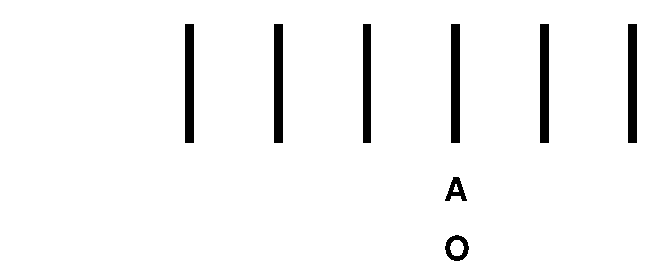
\includegraphics[scale=0.4]{moc}
% \end{SubFloat}%
% \vspace{-10pt}

\begin{SubFloat}{\label{fig:2c}Mapping to physical time}%
% \includegraphics[scale=0.4]{phy.pdf_t}
\scalebox{0.68}{\input{phy.pdf_t}}
\end{SubFloat}%
\caption{Simple SystemJ example and corresponding MoC}
\label{fig:2}
\end{figure}

The perfect synchrony hypothesis is ideal for programming the
synchronous sub-set of SystemJ. Unfortunately, every \textit{micro-step}
requires real-time to compute. Formally, execution of every micro-step
in the logical zero time requires $\delta$ physical time. Time for a
logical tick can thus be summarized as $\Delta = \mathcal{F} (\delta)$,
where $\mathcal{F}$ is some function dependent upon the
\underline{schedule}. We call $\Delta$ the reaction time. Depending upon
the amount of computation required and schedule, $\Delta$ can vary,
hence, in order to satisfy the implicit restriction imposed by the
synchrony hypothesis -- no input event \textit{from the environment} can
be missed -- one needs to calculate the \textit{Worst Case Reaction
  Time} (WCRT) and the resultant WCRT needs to be smaller than the time
between any two consecutive events on any input, else the synchrony
hypothesis is violated. Techniques for calculating the WCRT of
synchronous programs~\cite{boldt07} exist and this analysis is not the
focus of this paper. The opposite of the WCRT is the \textit{Best Case
  Reaction Time} (BCRT), we denote the WCRT and BCRT in
Figure~\ref{fig:2c} using \texttt{W} and \texttt{B},
respectively. Figure~\ref{fig:2c} shows a continuously running physical
clock (analogous to a clock in digital hardware), the numerical
annotations on the rising edge of the clock mark the logical ticks from
Figure~\ref{fig:2c}. The subscripts \texttt{s} and \texttt{e} for the
numbers show the start and end of the logical ticks, respectively. The
end of a logical tick and the start of the next logical tick happen
together. Figure~\ref{fig:2c} shows the mapping of the logical time to
the physical time. For example, the logical tick \texttt{1} starts at
the first rising edge and completes at the second rising edge of the
physical clock, whereas logical tick \texttt{4} starts at the $4^{th}$
rising edge, but finishes at the $6^{th}$ rising edge of the physical
clock. This difference can be accounted for by the Java computations
required when signal \texttt{A} is input by the environment (see
Figure~\ref{fig:2a}). This elasticity is inherent (and elegant) to both
Esterel and SystemJ.

% We now present a lemma with proof sketch (due to lack of space) that we
% require for the rest of the paper and is special to SystemJ, being a
% GALS language.

% \begin{lemma}
%   WCRT and BCRT analysis are invariant to values of conditional
%   expressions.
% \end{lemma}

% \begin{proof}
%   The physical time ($\delta$) taken by a conditional expression is at
%   best affected by the type rather than the value of the
%   conditional. Example, comparing the value of 2 floats might take
%   longer than comparing the value of 2 integer types on some given
%   platform. But, the time taken by the comparison instruction is
%   invariant to the value itself.
% \end{proof}

% \begin{lemma}
%   WCRT and BCRT analysis are invariant to channel communication.
% \end{lemma}
% \begin{proof}
%   LATER ....
% \end{proof}


%%% Local Variables: 
%%% mode: latex
%%% TeX-master: "paper"
%%% End: 

\section{Introducing real-time in SystemJ}
\label{sec:intr-real-time}

We introduce a single \textit{derived} (built from kernel constructs)
statement called \mbox{\texttt{delay (M..N)}} in the SystemJ language
for real-time control. The resolution of the delay statement is of
secondary concern and is dependent upon the execution platform.

\subsection{Semantics of the delay statement}
\label{sec:semant-delay-stat}

Given a SystemJ program: \texttt{delay (M..N); p}, where $M \in
\mathbb{Q}^{>0}$ and $N \in \mathbb{Q}^{>0}$, statement $p$ is executed
after real-time delay of $\tau$ units, such that, $M \leq \tau \leq N$.

We also introduce two variants of the derived statement \texttt{delay}.
\begin{enumerate*}
\item Given a SystemJ program \texttt{delay (M); p}, where $M \in
  \mathbb{Q}^{>0}$, statement $p$ is executed after real-time delay of
  $\tau$ units, such that, $M \leq \tau < \infty$. It is important to
  note that the lower bound of the delay construct $M$ is \textit{not}
  an exact delay, but rather the control is allowed to proceed to the
  next statement anytime after the delay of time $M$.
\item Given a SystemJ program \texttt{delay (M..M); p}, where $M \in
  \mathbb{Q}^{>0}$, statement $p$ is executed after real-time delay of
  $\tau$ units, such that, $M \leq \tau \leq M$. In this variant, the
  delay is exact.
\end{enumerate*}

The aforementioned variants are special cases of the general case
\texttt{delay (M..N)}.

\subsection{Rewriting the \texttt{delay} statement}
\label{sec:rewr-delay-stat}

The introduced \texttt{delay} construct is not a kernel construct, but a
\textit{derived} construct built from the kernel constructs
(Table~\ref{tab:1}) in SystemJ. Figure~\ref{fig:3} gives the rewrite of
the \texttt{delay} construct to kernel statements.

\begin{figure}[tb]
    \begin{minipage}{\textwidth}
      \begin{scriptsize}
\begin{verbatim}
trap(T){
 int x = 0;
 while(true){
  x = x + 1;
  pause;
  if(x == d) exit (T); //wait for "d" ticks
 } // d is the number of logical ticks calculated
} // by Algorithm 1
\end{verbatim}
      \end{scriptsize}
    \end{minipage}
    \caption{The rewrite of \texttt{delay} construct}
    \label{fig:3}
\end{figure}

The fundamental observation is that real-time is converted into logical
time via the \texttt{pause} construct. The rewrite basically maps the
physical notion of time back to the elegant logical notion of time. The
rewrite \textit{delays} a certain number of logical ticks, before
proceeding to the next statement. The number of logical ticks
\texttt{``d''} to \textit{delay} (Figure~\ref{fig:3}) is determined by
the compiler statically at compile time. The value of \texttt{d} is
intricately tied with the WCRT and BCRT of the program and hence the
execution platform.

\subsection{Finding the logical delay \texttt{d}}
\label{sec:find-logic-delay}

\begin{algorithm}[t!]
  \begin{minipage}{1.0\linewidth}
    \SetAlgoLined
    \KwData{WCRT, BCRT, $M \in \mathbb{Q}^{>0}$, $N \in \mathbb{Q}^{>0}$}
    \KwResult{d}
    let $l_1 \leftarrow \lceil \frac{M}{WCRT} \rceil$\;
    let $l_2 \leftarrow \lceil \frac{M}{BCRT} \rceil$\;
    let $u_1 \leftarrow \lfloor \frac{N}{WCRT} \rfloor$\;
    let $u_2 \leftarrow \lfloor \frac{N}{BCRT} \rfloor$\;
    let $F:(l_1,u_1) \rightarrow S_1$\;
    let $F:(l_2,u_2) \rightarrow S_2$\;
    let $D \leftarrow S_1 \cap S_2$\;
    \Return (some $d \in D$)\;
    \caption{Finding the value of \texttt{d}}
    \label{alg:1}
  \end{minipage}
\end{algorithm}

The computation of \texttt{d} is shown in Algorithm~\ref{alg:1}. This
algorithm is carried out for each CD (in SystemJ) or a synchronous
program individually. \textit{The fundamental observation is -- the
  reaction time for each logical tick is elastic -- varying only between
  the BCRT and the WCRT, thus any number of logical ticks \texttt{d}
  that map to the required real-time \texttt{delay} should be chosen in
  such a way that they are invariant to this elasticity.}

Our algorithm takes as input: WCRT, BCRT, and the lower and upper bounds
$M$ and $N$, respectively of the \texttt{delay} construct. We first
divide $M$ and $N$ with the BCRT and WCRT, respectively. This division
gives us the number of individual logical ticks required to delay the CD
(or synchronous program) by the real-time specification. We always
$ceil$ when dividing $M$ and $floor$ when dividing $N$ to make sure that
the resultant values are integers (in domain $\mathbb{N}^{>0}$) and
these functions guarantee that the resultant logical ticks result in
real-time delays between the required range $M-N$. Next, a function $F$
maps these calculated values to a set of equidistant integer points
(values) separated by a unit value -- these points represent all the
logical ticks running at the WCRT and the BCRT, respectively that
satisfy the real-time delay requirements. The intersection of these two
sets gives all the logical ticks that satisfy the real-time requirements
invariant of the logical time and its elasticity.

Let us revisit our motivating example to illustrate the algorithm. From
Figure~\ref{fig:1} we know that $M$ is 50.3 ms and $N$ is 200.3 ms,
respectively. Let the WCRT and BCRT be: 0.112 ms and 0.0334 ms,
respectively. Thus, the algorithm proceeds as follows:

\begin{enumerate*}
\item $l_1 \leftarrow \lceil 50.3/0.112 \rceil$ and $u_1 \leftarrow
  \lfloor 200.3/0.112 \rfloor$. $l_1 = 450$ and $u_1 = 1788$. We first
  calculate the logical ticks that are always running at the WCRT and
  satisfy the required real-time delay.
\item $l_2 \leftarrow \lceil 50.3/0.0334 \rceil$ and $u_2 \leftarrow
  \lfloor 200.3/0.0334 \rfloor$. $l_1 = 1506$ and $u_1 = 5997$. We do
  the same for the BCRT case.
\item $S_1 = [450..1788]$ and $S_2 =[1506,5997]$. We then map the
  resultant bounds to linear points. Sets $S_1$ and $S_2$ represent
  logical ticks that running at the WCRT and BCRT, respectively always
  satisfy the required real-time constraints.
\item $D = S_1 \cap S_2$, $D = [1506,1788]$. Finally, the intersection
  of the two sets gives the set $D$ from which we can choose any value
  for \texttt{d}.
\end{enumerate*}

The resultant value for \texttt{d} gives the number of logical ticks,
which can run at any physical clock-speed, bounded by the BCRT and the
WCRT of the program and still result in the desired real-time delay. We
think this is an elegant solution, because the technique provides
hard-real time guarantees while preserving the essence (elastic logical
tick) of synchronous and GALS programming prescribed by SystemJ and
Esterel style languages. Moreover, this technique considers non
maximal-parallelism, i.e., the delays in logical ticks is calculated
after scheduling of CDs or synchronous programs has been performed. To
our knowledge we are the first to do so.

\subsection{Extending the technique to variants of \texttt{delay}}
\label{sec:extend-tehcn-vari}

\paragraph{The \texttt{delay(M)} construct}
\label{sec:extend-techn-vari}

The \texttt{delay(M)} variant is easily accommodated in the
technique. All one needs to do is find the set $S_1$ and choose a value
from this set.

\paragraph{The \texttt{delay(M..M)} construct}
\label{sec:extend-techn-vari}

The \texttt{delay(M..M)} variant is a little more interesting. Like
before we find sets $S_1$ and $S_2$, and find the intersection of the
two sets to get the value of \texttt{d}. It is possible (and often
likely, as suggested by our experiments in
Section~\ref{sec:experimental-results}) that the resultant set $D$ is
empty (also possible in the case of \texttt{delay(M..N)}, but never
possible in case of \texttt{delay(M)}). In such a case, we automatically
\textit{relax} the upper bound of the \texttt{delay} statement.

\paragraph{Relaxation of the upper real-time bound}
\label{sec:over-appr-relax}

The relaxation technique is shown in Algorithm~\ref{alg:2}.
  
\begin{algorithm}[t!]
  \begin{minipage}{1.0\linewidth}
    \SetAlgoLined
    \KwData{$S_2$, $D$, WCRT}
    \KwResult{d}
    \If {$D = \emptyset$} {
      let $j_{0}$ be the first element of set $S_2$, s.t., $|S_2|=Q$\;
      \ShowLn let $N \leftarrow WCRT \times j_0$\;
      let $d \leftarrow j_0$\;
    }
    \Return d\;
    \caption{Calculating the minimum relaxation of the upper real-time
      bound}
    \label{alg:2}
  \end{minipage}
\end{algorithm}


This algorithm results in the smallest relaxation required for the
real-time delay to be satisfied. The algorithm takes as input the WCRT
and set $S_2$, recall that set $S_2$ represents the logical ticks
required to satisfy the real-time requirement at the BCRT. We take the
very first value from set $S_2$ and multiply it with the WCRT to get the
relaxation $N$. The first element of set $S_2$ is returned as the
logical tick delay \texttt{d}.

The fundamental observation is that we have to delay for a minimum of
$M$ units of real-time, hence, under-approximation is out of
question. We can still over-approximate, but to reduce the resultant
error, we should over-approximate by least possible value, which is the
lower bound of set $S_2$. Thus, the lower bound is considered to be the
only element shared between the two sets $S_1$ and $S_2$ and
accordingly, the upper real-time bound is relaxed by the multiplication
of WCRT and the first element of set $S_2$.


\subsection{Programming using the delay construct}
\label{sec:progr-using-delay}

In this section we provide a number of examples to show the different
types of real-time programming paradigms that can be incorporated into
the GALS (and its sub-set synchronous) programming model.

\subsubsection{Non-deterministic time}
\label{sec:non-determ-time}

Many real-world systems require non-deterministic timing
constructs. Where the exact real-time delay is not known or should not
be known apriori. One such system is our motivating example -- the human
response time system.

% Another is a printer-spooler example borrowed from timed
% CSP~\cite{Schneider:1999:CRT:555233}. The spooler and printer need to
% synchronize using channels. The printer might be unable to print
% depending upon the paper tray, similarly, spooler might take sometime
% to send the job depending upon its size. Such real-time constraints
% can be modeled in SystemJ as below:

% \begin{scriptsize}
  
% \begin{verbatim}
% {await (job); delay (2..10 ms);  //SPOOLER CD
%  send mid(job) delay (1ms);}
% ><
% {receive mid; delay(1..30 ms); //PRINTER CD
%  emit print(#mid);}
% \end{verbatim}
% \end{scriptsize}

\subsubsection{Timeout}
\label{sec:timeout}

There are many instances when one would like to wait on an input from
environment for only a specified amount of time. This can be programmed
as:
% \begin{scriptsize}
\begin{verbatim}
// timeout after 1ms.
trap(T){{await(A);}||{delay(1..1 ms);exit(T);}}
\end{verbatim}
% \end{scriptsize}

\subsubsection{Periodic reactions}
\label{sec:periodic-reactions}

A reaction, or a whole CD, can be programmed to run periodically like
so:

% \begin{scriptsize}
\begin{verbatim}
while(true) { delay ((1..1)ms); emit S; 
 //do something }
\end{verbatim}
% \end{scriptsize}
A periodic reaction (or CD) requires special consideration. Since the
delay statement is converted into \texttt{pause} constructs. One should
not introduce extra \texttt{pause} constructs when building periodic
reactions (or CDs). This is essential since introducing additional
pauses would introduce more logical ticks.

\subsubsection{Interaction of preemption and delays}
\label{sec:inter-preempt-delays}

Preemption plays an important role in reactive languages. One needs to
carefully consider the interplay of \texttt{delay} semantics with the
preemption semantics of reactive languages. Previous attempts at
incorporating delays (using external timers) have only been partially
successful, because of the complex interplay between real-time and
preemption. Consider the simple example below, which models real-time
using external timers as in~\cite{rsh94}.

% \begin{scriptsize}
\begin{verbatim}
suspend{S} {emit START_TIMER(10); await (TIMER); 
 emit O1;}
\end{verbatim}
% \end{scriptsize}

As identified in~\cite{Bourke2009a} the \texttt{suspend} does not play
well with the external timer. The above program sends a signal to an
external timer and waits for 10 ms to pass by. Consider what happens
when signals \texttt{S} and \texttt{TIMER} occur in the same logical
tick, the \texttt{await} statement is never executed (due to suspend)
and hence, we enter a deadlock. Such problems are completely avoided in
our technique, because we convert the real-time delays into logical
delays (\texttt{pause} constructs), which interact well with preemption.

\subsubsection{Interaction of channel communication and delays}
\label{sec:inter-chann-comm}

Channels, used for communication between reactions in asynchronously
running CDs, are an addition in the SystemJ language. Like interaction
of preemption and delays, conversion of real-time delays to logical
ticks also interacts well with channel rendezvous, because the semantics
of interaction are well defined~\cite{amal10}. More importantly, we need
to consider the interplay of channel communication and WCRT/BCRT
analysis. Since, channel communication does not stop logical time
(see~\cite{amal10}) WCRT/BCRT are unaffected by channel
communication. % The response time to input signals \textit{is} though!
% But, we are unconcerned with the response time, analysis in this paper
% and it remains a future research avenue.

%%% Local Variables: 
%%% mode: latex
%%% TeX-master: "paper"
%%% End: 



\section{Experimental results}
\label{sec:experimental-results}

\begin{center}
\scalebox{0.9}{
\begin{tabular}{|c| c | c | c | c | c | c | c |}
	\cline{4-8}
	\multicolumn{3}{c|}{}											& HRTCS 		& Motor 		  & Robot 			  & AECS/CD1  		   & AECS/CD2\\ \hline
	\multirow{12}{*}{JOP} 		& \multicolumn{2}{|c|}{BCRT} 		&0.0334 ms 		& 0.0361 ms		  & 0.0325 ms		  & 0.1683 ms		   & 0.1881 ms\\ \cline{2-8}   
								& \multicolumn{2}{|c|}{WCRT} 		&0.1120 ms 		& 0.1116 ms		  & 0.0601 ms		  & 0.7147 ms		   & 1.0115 ms\\ \cline{2-8} 
								& \multirow{2}{*}{Delay 1}	 & M..N &50.3-200.3 ms 	& 2.4-7.4772 ms	  & 1230-2274.0263 ms & 10000-42473.2197 ms& 10000-53772.0045 ms \\ \cline{3-8} 
								&			   & d			 		&1506-1787  	& 67 			  & 37861			  & 59427		       &53160\\ \cline{2-8}
								& \multirow{2}{*}{Delay 2}	 & M..N & 	N/A 		& 1.667-5.2452 ms & N/A				  & N/A 			   &10000-53772.0045 ms\\ \cline{3-8} 
								&			   & d			 		& 	N/A	 		& 47			  & N/A				  & N/A       		   &53160\\ \cline{2-8}
								& \multirow{2}{*}{Delay 3}	 & M..N & 	N/A	 		& 0.05-0.2232 ms  & N/A				  & N/A       		   &N/A\\ \cline{3-8} 
								&			   & d			 		& 	N/A	 		& 2		      	  &	N/A				  & N/A       		   &N/A\\ \cline{2-8}
								& \multirow{2}{*}{Delay 4}	 & M..N & 	N/A	 		& 0.3-1.0044 ms   & N/A				  &	N/A       		   &N/A\\ \cline{3-8} 
								&			   & d				 	& 	N/A	 		& 9				  & N/A				  &	N/A      		   &N/A\\ \cline{2-8}
								& \multirow{2}{*}{Delay 5}	 & M..N & 	N/A	 		& 0.733-2.3436 ms & N/A				  &	N/A      		   &N/A\\ \cline{3-8} 
								&			   & d			 		& 	N/A	 		& 21 			  &	N/A				  & N/A      		   &N/A\\ \hline
	\multirow{12}{*}{TP-JOP} 	& \multicolumn{2}{|c|}{BCRT} 		&0.0028 ms 		& 0.0060 ms		  & 0.0011 ms		  & 0.0532 ms		   & 0.0292 ms\\ \cline{2-8}   
								& \multicolumn{2}{|c|}{WCRT} 		&0.0329 ms 		& 0.0393 ms		  & 0.0361 ms		  & 0.5072 ms		   & 0.8388 ms\\ \cline{2-8} 
								& \multirow{2}{*}{Delay 1}	 & M..N &50.3-600.3 ms 	& 2.4-15.6265 ms  & 1230-42317.8276 ms& 10000-95358.8578 ms& 10000-287757.9834 ms \\ \cline{3-8} 
								&			   & d			 		&18209-18232 	& 398 			  & 1171429			  & 188015		       &343054\\ \cline{2-8}
								& \multirow{2}{*}{Delay 2}	 & M..N & 	N/A 		& 1.667-10.8757 ms& N/A				  & N/A 			   &10000-287757.9834 ms\\ \cline{3-8} 
								&			   & d			 		& 	N/A	 		& 277			  & N/A				  & N/A       		   &343054\\ \cline{2-8}
								& \multirow{2}{*}{Delay 3}	 & M..N & 	N/A	 		& 0.05-0.3534 ms  & N/A				  & N/A       		   &N/A\\ \cline{3-8} 
								&			   & d			 		& 	N/A	 		& 9		      	  &	N/A				  & N/A       		   &N/A\\ \cline{2-8}
								& \multirow{2}{*}{Delay 4}	 & M..N & 	N/A	 		& 0.3-1.9631 ms   & N/A				  &	N/A       		   &N/A\\ \cline{3-8} 
								&			   & d				 	& 	N/A	 		& 50			  & N/A				  &	N/A      		   &N/A\\ \cline{2-8}
								& \multirow{2}{*}{Delay 5}	 & M..N & 	N/A	 		& 0.733-4.79 ms   & N/A				  &	N/A      		   &N/A\\ \cline{3-8} 
								&			   & d			 		& 	N/A	 		& 122 			  &	N/A				  & N/A      		   &N/A\\ \cline{2-8}
	\hline
\end{tabular}
}
\end{center}


aa

%%% Local Variables: 
%%% mode: latex
%%% TeX-master: "paper"
%%% End: 



\section{Discussion}
\label{sec:disc-perc-limit}

We dedicate this section to discuss the details of the wait construct
semantics, their usage and the advantages and limitations of our
proposed technique to introducing these real-time constructs in a
reactive setting.

\subsection{Programming using the wait\_exactly construct -- the
  periodic reactions}
\label{sec:progr-using-delay}

% All three delay constructs are useful for programming real systems. % The
% first form of the delay construct $delay(M..N)$ is used to program
% non-determinism like in the HRCTS system and a real printer-spooler
% embedded system, etc. The second form is useful for programming low
% priority periodic tasks.

% \subsubsection{Non-deterministic time}
% \label{sec:non-determ-time}

% Many real-world systems require non-deterministic timing
% constructs. Where the exact real-time delay is not known or should not
% be known apriori. One such system is our motivating example -- the human
% response time system (HRTCS). Another one we presented was a real
% printer-spooler embedded controller in
% Section~\ref{sec:experimental-results}.

% \subsubsection{Timeout}
% \label{sec:timeout}

% There are many instances when one would like to wait on an input from
% environment for only a specified amount of time. This can be programmed
% as:

% \begin{figure}[h!]
%   \centering
% 			\vspace{-10pt}
% 			\begin{lstlisting}[style=sysj,basicstyle=\normalsize\ttfamily,morekeywords={await,emit,trap,pause,exit,delay}]
% // timeout after 1ms.
% trap(T){{await(A);}||
%         {delay(1 ms);exit(T);}}
% \end{lstlisting}
%   \caption{Programming low priority timeout tasks with delay statements}
%   \label{fig:timeout}
% 			\vspace{-10pt}
% \end{figure}

% In the above case, the program waits for signal \texttt{A} from the
% environment for \textit{at least} \texttt{1 ms}, but it may wait longer
% if other reactions/CDs are scheduled for execution. This second variant
% of delay statement is very useful for programming low priority tasks.

% \subsubsection{Periodic reactions}
% \label{sec:periodic-reactions}

% The third variant is useful for hard-real time guarantees, e.g., a
% reaction, or a whole CD, can be programmed to run periodically like so:

\begin{figure}[h!]
  \centering
	\vspace{-10pt}
        \begin{lstlisting}[style=sysj,basicstyle=\normalsize\ttfamily,morekeywords={emit,trap,pause,exit,wait_exactly}]
          while(true){wait_exactly (1 ms); emit S; //do something
          }
 \end{lstlisting}
  \caption{Programming periodic tasks with wait\_exactly statement}
  \label{fig:periodic}
	\vspace{-10pt}
\end{figure}

The program in Figure~\ref{fig:preemp}, reproduced from
Section~\ref{sec:progr-using-exact}, is supposed to emit signal
\texttt{S} every \texttt{1 ms}. Such periodic reactions (or CDs) require
special consideration, like any other real-time periodic task. One
should be aware of the interaction of wait and other \texttt{pause}
constructs in the body of the reaction (or CD). For example, consider
the (perceived) periodic program and its rewrite below.

\begin{figure}[h!]
  \centering
  \begin{SubFloat}{\label{pp:a}Original program}
    \centering
			\begin{lstlisting}[style=sysj,basicstyle=\normalsize\ttfamily,morekeywords={emit,trap,pause,exit,wait_exactly}]
while(true) {
 wait_exactly(1 ms);
 //extra pause
 pause;
 emit S;
}
\end{lstlisting}
\end{SubFloat}
\hspace{9pt}
  \begin{SubFloat}{\label{pp:b}Rewritten program}
			\begin{lstlisting}[style=sysj,basicstyle=\normalsize\ttfamily,morekeywords={emit,trap,pause,exit,delay}]
while(true) {
 while(true) { 
  trap(T) {
   int x = 0;
   while(true) {
    x = x + 1;
    pause;
    if (x == d)
     exit(T);
   }
  }
  //extra pause
  pause;
  emit S;
 }
}
\end{lstlisting}
  \end{SubFloat}
\caption{Extra pause statements in periodic tasks}
  \label{fig:periodic2}
\end{figure}

The system designer needs to be aware that just introducing a wait
construct does not make the reaction (or CD) periodic. The program on
the left does \textit{not} emit signal \texttt{S} every \texttt{1 ms},
because of the extra \texttt{pause} statement. Introducing additional
pauses introduces more logical ticks, consequently increasing the
real-time wait constructs. Static analysis techniques from real-time
community can be used to automatically determine the wait specification,
in such cases, but describing these techniques is out of the scope of
this work.

\subsection{Need for time analyzable platforms}
\label{sec:need-time-analyzable}

The proposed solution relies on time analyzable platforms, i.e.,
platforms where WCRT and BCRT can be calculated using static analysis
tools. Many might consider this to be too much of a restriction. In this
section we debunk this \textit{perceived} disadvantage.

\subsubsection{Interaction of timers and reactive constructs}
\label{sec:inter-timers-react}

As mentioned previously, the proposed solution might need
over-approximation techniques (Algorithm~\ref{alg:2}) to guarantee
timing requirements (cf. Section~\ref{sec:extend-tehcn-vari}). This
might give the readers an impression that timer based solution proposed
for standard real-time operating systems should be utilized for
GALS/synchronous programs. This is a fallacy. Bourke et
al~\cite{Bourke2009a} have investigated this technique
unsuccessfully. We elaborate upon the interplay of timers and reactivity
to make the problem of using timers explicit.

Preemption plays an important role in reactive languages. One needs to
carefully consider the interplay of wait constructs semantics with the
preemption semantics of reactive languages. Previous attempts at
incorporating delay (using external timers) have only been partially
successful, because of the complex interplay between real-time and
preemption. Consider the simple example below, which models real-time
using external timers as in~\cite{rsh94}.

\begin{figure}[h!]
  \centering
	\vspace{-10pt}
		\begin{lstlisting}[style=sysj,basicstyle=\normalsize\ttfamily,morekeywords={emit,trap,pause,exit,delay,suspend}]
suspend(S) {
 emit START_TIMER(10); 
 await (TIMER);emit O1;
}
		\end{lstlisting}
  \caption{Interaction of preemption and external timers}
  \label{fig:preemp}
	\vspace{-10pt}
\end{figure}

As identified in~\cite{Bourke2009a} \texttt{suspend} does not play well
with the external timer. The above program sends a signal to an external
timer and waits for 10 ms to pass by. Consider what happens when signals
\texttt{S} and \texttt{TIMER} occur in the same logical tick, the
\texttt{await} statement is never executed (due to suspend) and hence,
we enter a deadlock. Such problems are completely avoided in our
technique, because we convert the real-time wait constructs into logical
waits (\texttt{pause} constructs), which interact well with preemption.
Furthermore, synchronous/GALS languages have always been targeted at
real-time analyzable platforms and constrained
environments~\cite{DBLP:journals/pieee/SifakisTY03,boldt07}. One can use
our technique within such a setting with ease.

\subsubsection{The timer resolution problem}
\label{sec:resolution-real-time}

\begin{figure}[h!]
  \centering
	\vspace{-10pt}
		\begin{lstlisting}[style=sysj,basicstyle=\normalsize\ttfamily,morekeywords={emit,trap,pause,exit,delay,suspend}]
{
 //reaction R1
 emit START_TIMER(1 ms); 
 await (TIMER);emit O1;
}
||
{
 //reaction R2
 // do something
}
		\end{lstlisting}
  \caption{Resolution of external timers}
  \label{fig:resolution}
	\vspace{-10pt}
\end{figure}

There is yet another problem with timer based systems. Let us consider
the program in Figure~\ref{fig:resolution}. On a cursory look this
example should work fine. An external timer is started in reaction R1,
which counts down from 1 ms. Once this time has elapsed a signal
\texttt{TIMER} is generated from this external timer, which should emit
O1 in turn. There is no \texttt{suspend} construct encapsulating the
timer and hence all seems fine. Let us now consider what happens to the
whole CD, including reaction R2; while reaction R1 is waiting for the
\texttt{TIMER} signal, reaction R2 is making progress. Input signals can
only be captured from the environment at the logical tick boundaries
(cf. Section~\ref{sec:mapping-logical-time}). In
Figure~\ref{fig:resolution}, reaction R2 determines the length of the
tick, because it is performing the heavier computation. Consider what
happens if the external timer generates the \texttt{TIMER} signal, but
the system is still performing computation and the logical tick has not
yet finished -- we \textit{miss} this \texttt{TIMER} signal from the
environment. Thus, even in the absence of the \texttt{suspend}
construct, we are not guaranteed that the program will capture the
external timer signal. In fact, the WCRT needs to be smaller than 1 ms
for the above program to perform as expected. But, this again implies
need for a time analyzable platform even when using external timers.

In general we observe that the WCRT determines the lowest resolution of
any real-time construct whether it be external timer independent, like
the proposed technique, or external timer dependent, like above. This
discovery is one of the key insights for proposing the solution
described in this paper.

% \subsection{Other semantic discussion}
% \label{sec:other-semant-dissc}

\subsection{Interaction of channel communication and wait constructs}
\label{sec:inter-chann-comm}

Channels, used for communication between reactions in asynchronously
running CDs, are an addition in the SystemJ language. Like interaction
of preemption and waits, conversion of real-time wait constructs to
logical ticks also interacts well with channel rendezvous, because the
semantics of interaction are well defined~\cite{amal10}. More
importantly, we need to consider the interplay of channel communication
and WCRT/BCRT analysis. Since, channel communication does not stop
logical time (see~\cite{amal10}) WCRT/BCRT are unaffected by channel
communication. % The response time to input signals \textit{is} though!
% But, we are unconcerned with the response time, analysis in this paper
% and it remains a future research avenue.

% \subsubsection{Interaction of synchronous parallelism and delay}
% \label{sec:inter-synchr-parall}

% {\color{red}Maybe we should talk about how the control flow in other
%   reactions and CDs is not affected by the delay statement.}



%%% Local Variables: 
%%% mode: latex
%%% TeX-master: "paper"
%%% End: 

% \vspace{-15pt}
\section{Related work}
\label{sec:related-work}


A number of studies have been performed when it comes to integrating
real-time directly as a programming construct in GALS (and its subset
synchronous) reactive languages. The most prominent works in this area
are by Shyamsundar~\cite{rsh94} and Bourke et
al.~\cite{Bourke2009a}. Shyamsundar incorporates real-time using
external timers in \textit{Communicating Reactive Processes} (CRP),
which like SystemJ is an extension of synchronous language Esterel to
asynchorny. But, as mentioned in Section~\ref{sec:inter-preempt-delays},
external timers do not interact well with preemption constructs in these
languages. Bourke et al. introduce real-time as first class constructs
in the Esterel language. They like us provide real-time \texttt{delay}
as first class Esterel programming constructs, and translate them into
Esterel kernel constructs. But, unlike us they do not translate delays
into \texttt{pause} constructs directly. Instead, logical ticks are
generated by using abstract notion of \texttt{event} and \texttt{sample}
platform dependent timers. This notion makes it a complex and inflexible
solution since the number of platform timers with certain resolutions
need to be determined and present on the system for the solution to be
realizable. Moreover, non-deterministic real-time delays and integration
with non-maximal parallelism is not studied at all. Our solution does
not require external timers (like~\cite{rsh94}) or logical notion of
timers (like~\cite{Bourke2009a}). In our solution we calculate the delay
in logical ticks \textit{after} allocation and scheduling, it gives the
compiler developers the chance to optimize for many different criteria
such as computation time, energy, power, etc, without worrying about or
violating the real-time delay specification.

Other works such as Quartz~\cite{glog02} and Bertin et
al.~\cite{Bertin:2000:TVR:1947412.1947439}, also incorporate delay
statements in Esterel using \texttt{pause} and special \textit{pragmas}
(annotations), respectively.  The Quartz solution is targeted at
studying timing properties using model checkers rather than
implementation, like us. The solution introduced by Bertin et
al.~\cite{Bertin:2000:TVR:1947412.1947439} translates real-time pragmas
into Timed automata~\cite{alur94} for model-checking real-time
deadlines. Our solution on the other hand removes all continuous time
elements and produces single discrete time model thereby making the
solution amenable to existing functional and real-time verification
tools developed for reactive languages and more in the spirit of logical
time. Finally, a major difference between Bertin et al. and our approach
is that their approach requires programmers to annotate the time taken
by `C' code fragments manually, this is extremely error prone, we use
static low-level program analysis to find out such times automatically.


%%% Local Variables: 
%%% mode: latex
%%% TeX-master: "paper"
%%% End: 



\section{Conclusion}
\label{sec:concl-future-work}

In this paper we have described a novel way to introduce real-time in
\textit{Globally Asynchronous Locally Synchronous} (GALS) languages, in
particular SystemJ, and their subset the synchronous languages like
Esterel. The fundamental idea is to convert real-time delay into logical
delays (\texttt{pause} construct) that interact well with rest of the
constructs in these languages, especially, preemption and channel
communication. We do \textit{not} need or use external timers to
introduce these real-time delays, instead we depend upon an underlying
platform that is timing analyzable, thereby resolving the problems of
interaction between external timers and preemption. Moreover, we also do
not require specific timer resolutions, thereby making our solution
elegant (in the spirit of GALS/synchronous programming) and flexible. We
rewrite the delay construct into reactive kernel constructs, calculate
the \textit{Worst} and \textit{Best} case reaction times and then
determine \textit{delay} \texttt{d}, number of logical ticks, which is
invariant to the \textit{elasticity} of logical time. To our knowledge
we are the first to introduce precise and imprecise delays in such
languages and show their usefulness in designing real-world systems.


%%% Local Variables: 
%%% mode: latex
%%% TeX-master: "paper"
%%% End: 


\bibliographystyle{IEEEtran}
\bibliography{main}
\end{document}


